\section{Description technique}

Comme cité précédemment, notre application a été codé à l'aide de la librairie JavaFX. Ainsi, toute notre implémentation technique est basée sur cette dernière.

\subsection{Structure}
\subsubsection{Structure de JavaFX}
Notre application se base sur la structure officielle d'une application JavaFX, qui se prête parfaitement à notre type d'application. Sa compréhension est essentielle pour discuter de l'architecture de notre logiciel.
\par
Les trois point-clés sont la notion de \gls{stage}, de \gls{scene} et de \gls{scene_graphe}. Le Stage est le container haut-niveau d'une application JavaFX \cite{javadoc_stage}. Il doit contenir tout le contenu d'une fenêtre. La Scene est le container pour un Scene Graph. Chaque scène doit avoir un et un seul nœud racine du Scene Graph \cite{javadoc_scene}.
\par
<<<<<<< HEAD
Le Scene Graph est une structure en arbre qui garde une représentation interne des éléments graphiques de l'application. En tout temps, il sait quels éléments afficher, quels zones de l'écrans doivent être rafraîchies, et comment le faire de la manière la plus efficace \cite{javadoc_scene_graphe}. 	
=======
Le Scene Graph est une structure en arbre qui garde une représentation interne des éléments graphiques de l'application. En tout temps, il sait quels éléments afficher, quels zones de l'écrans doivent être rafraîchies, et comment le faire de la manière la plus efficace.
>>>>>>> c8ce2aecdad1067740a9e64c7dedafd99fc3099e
\begin{figure}[H]
	\caption{Représentation du Scene Graph de JavaFX. Source: documentation Oracle \cite{javadoc_scene_graphe}}
	\centering
	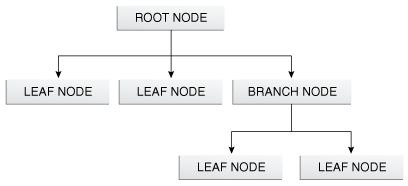
\includegraphics[scale=0.6]{scene_graphe_1.png}
	\label{fig:scene_graphe_1}
\end{figure}
Comme ont peut le voir sur la figure \ref{fig:scene_graphe_1}, chaque nœud de l'arbre du Scene Graph appartient à la hiérarchie de la classe Node. De plus chacun de ces nœuds est soit une feuille (ne pouvant pas contenir d'enfants), soit une branche (pouvant alors contenir des enfants).
\par
Cette structure particulière permet donc de créer facilement des interfaces graphiques, car il suffit que chaque élément visuel de notre application soit un objet (spécialisé ou non) d'une classe héritant de Node pour l'affichage de cet élément soit géré automatiquement par JavaFX.
\par
Pour beaucoup de nos composants, nous avons donc spécialisé une des classes offertes par JavaFx proposant la fonctionnalité recherchée, en y ajoutant les comportements dont nous avions besoin. Il sont ensuite ajouté au Scene Graph de la scène principale, et nous pouvons ainsi construire notre application.


\subsection{Serialisation}
\label{sec:serialisation}
En Java, la sérialisation s'effectue à l'aide de l'interface \og Serializable \fg{}. Par conséquent, chaque classes de Java implémentant cette dernière telle que \og String \fg{}, peut être sérialisé et désérialisé à volonté. Cependant, la majorité des classes JavaFX n'implémente pas cette interface. En effet, cette librairie utilise grandement des mécanismes et des liaisons dynamiques tel que les listeners qui sont pour l'instant des sous-systèmes non-sérialisable. C'est pourquoi, JavaFX contient peu d'objet sérialisable.

Pour combler ce manque, nous devons nous même implémenter la sérialisation des classes JavaFX que nous sommes susceptible d'utiliser.

\begin{figure}[h]
    \caption{Diagramme de la sérialisation simplifié}
    \centering
    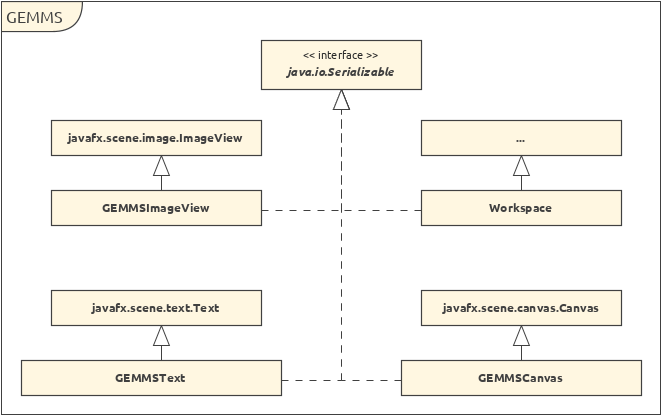
\includegraphics[scale=0.6]{serialisation_diagram.png}
    \label{fig:seri_diag}
\end{figure}

Sur la figure \ref{fig:seri_diag}, nous pouvons voir un diagramme simplifié de l'implémentation de la sérialisation. Dans notre application, nous allons utilisé des classes de base telles que ImageView, Text, Canvas, Color, etc. Nous devons donc spécialiser ces classes afin qu'elles puissent implémenter l'interface \og Serializable \fg{}. Toutefois, certaines classes comme \og Color \fg{} ne sont malheureusement pas spécialisable. Il faut donc sérialiser les paramètres un par un à l'aide des accesseurs et mutateurs de cette dernière.

Étant donné que les classes JavaFX possèdent énormément de fonctionnalités, sérialiser l'entier de celles-ci nous demanderait beaucoup trop de temps. C'est pourquoi nous nous contentons uniquement des paramètres utilisés au sein du projet tel que la largeur, la hauteur, la position, etc.

\lstinputlisting[language=Java, caption=Exemple de sérialisation]{./src/serialisation.java}

Bien que la sérialisation soit possible, ceci engendre des contraintes et des pertes de performances. Par exemple, les classes spécialisées ne peuvent plus étendre d'une classe commune et bénéficier de ses méthodes. De plus, les objets comme Canvas et ImageView devront sérialiser pixel par pixel, ce qui peut être long et volumineux selon la taille.

\subsection{Sauvegarde}
La sauvegarde d'un document utilise la sérialisation des objets. Comme mentionné précédemment, la sérialisation de certaines classes peut être volumineux. Ainsi, les données sont compressées dans le format GZIP.

\subsection{Workspace et liste des calques}
<<<<<<< HEAD
Le \gls{workspace} correspond à l'espace de travail d'un Document GEMMS. Workspace est une classe personnalisée héritant de la classe StackPane de JavaFX. Il s'insère donc dans le graphe de scène de JavaFX. 
=======
Le Workspace correspond à l'espace de travail d'un Document GEMMS. Le Workspace est une classe personnalisée héritant de la classe StackPane de JavaFX. Il s'insère donc dans le graphe de scène de JavaFX.
>>>>>>> c8ce2aecdad1067740a9e64c7dedafd99fc3099e
\subsubsection{Structure d'un Workspace}
Chaque document ouvert possède un objet Workspace permettant à l'utilisateur de manipuler le contenu du fichier. Il est constitué de couches comme représenté sur la figure \ref{fig:workspace_representation}.


\begin{figure}[H]
	\caption{Représentation des couches du Workspace}
	\centering
	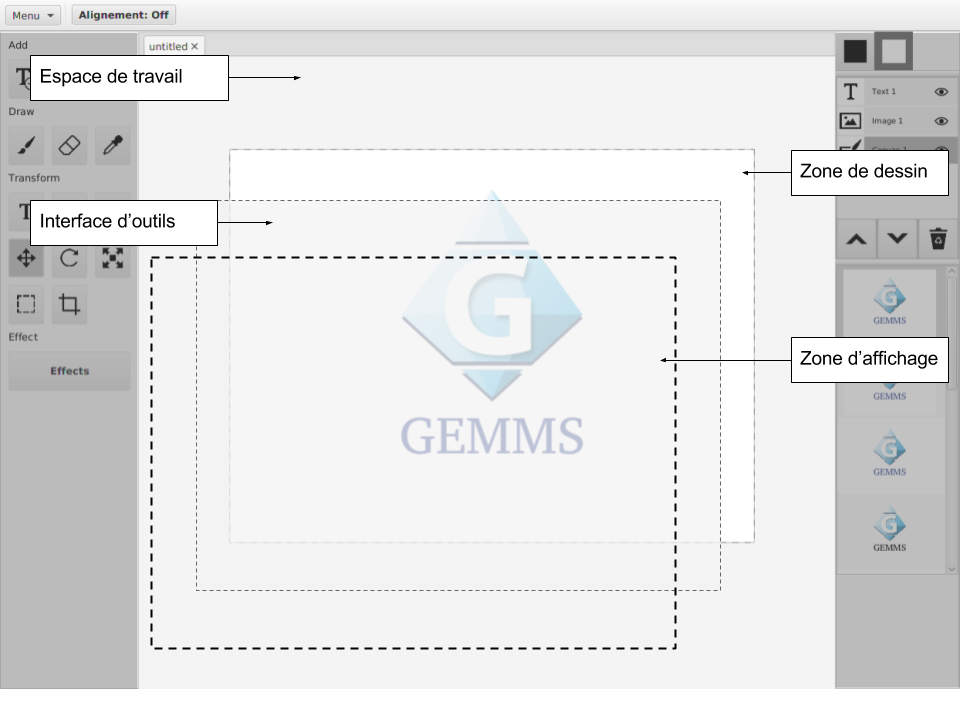
\includegraphics[scale=0.5]{workspace_schema.png}
	\label{fig:workspace_representation}
\end{figure}

L'espace de travail (Workspace) est un container contenant deux enfants (au sens de l'arbre de JavaFX): une zone de dessin (une branche du graphe de scène) ou seront ajoutés tous les calques créés et modifiés par l'utilisateur, et une interface des outils permettant de dessiner les retours visuels des outils (comme le curseur du pinceau par exemple). Tous deux sont de type AnchorPane, car cela permet de positionner leurs enfants selon des coordonnées (x, y).
\par
La zone d'affichage correspond à un masque appliqué à l'espace


\subsection{Copier-coller}
Deux façon d'aborder le copier-coller ont été implémentées : la première consiste à enregistrer dans le presse-papier un ou des calques sélectionnés, la seconde consiste à enregistrer uniquement la partie sélectionnée et visible à l'écran.

Trois procédés sont à l'origine de cette fonction de l'application : le snapshot, le viewport et la sérialisation.

\subsubsection{Snapshot}
Le snapshot est un outil proposé par JavaFX qui permet d'effectuer une «capture» d'un élément ou un groupe d'élément. C'est ce qui nous intéresse lorsque l'on fait une copie d'une zone sélectionnée de l'écran. L'image ainsi capturée est alors écrite sur un \texttt{GEMMSCanvas} qui est sérialisé et enregistré dans le presse-papier.

\subsubsection{Viewport}
La notion de Viewport intervient dans le cas d'un snapshot. Elle permet de définir une «fenêtre» de capture rectangulaire à laquelle se restreindra le snapshot, on la passe en paramètre au moment d'effectuer ce dernier.

Ce mécanisme est utilisé quand on copie une zone sélectionnée de l'espace de travail (voir \ref{sec:selection} pour la sélection). Les coordonnées de la sélection (position et taille) sont récupérées et utilisées pour créer un viewport. Le défi principal a été de gérer le système de coordonnées de JavaFX. En effet, chaque noeud possède son propre système de coordonnées et un point de ce noeud peut être exprimé selon le système de coordonnées local au noeud, selon le système du parent direct du noeud ou encore selon le système de la fenêtre, de l'écran etc.

La notion a maîtriser ici est d'exprimer au viewport ses dimensions dans le système de coordonnées du parent du noeud sur lequel on effectue le snapshot. Une fois cette notion comprise, le snapshot est restreint au viewport (et donc à la sélection) et le comportement voulu est adopté.

Il reste ensuite à écrire l'image capturée sur un \texttt{GEMMSCanvas} qui sera affiché par la suite dans l'espace de travail.

\subsubsection{Sérialisation}
Le presse-papier ne permet d'enregistrer que des données textuelles, il faut donc sérialiser le ou les calques qui seront stockés dans le presse-papier. Pour plus de détails sur la sérialisation, voir la section \ref{sec:serialisation}.

\subsubsection{Coller le contenu du presse-papier}
Le collage consiste à désérialiser le contenu du presse-papier et à insérer dans le Workspace courant le ou l'ensemble de calques désérialisés.

\subsection{Historique}
L'historique des actions effectuées se base principalement sur deux concepts : la sérialisation et le patron de conception «Observable» comme l'indique la figure \ref{fig:hist_uml}.

\begin{figure}[h]
    \caption{Diagramme de l'historique simplifié}
    \centering
    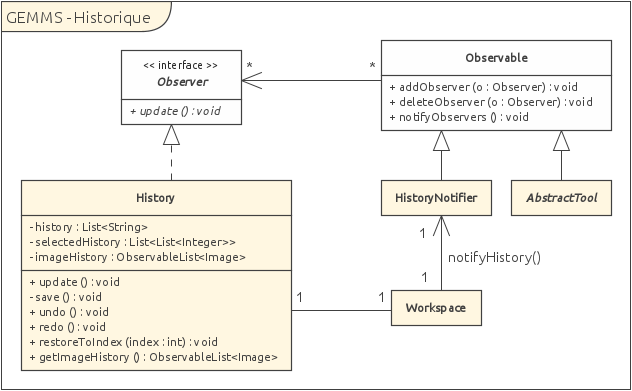
\includegraphics[scale=0.6]{history_uml.png}
    \label{fig:hist_uml}
\end{figure}

Après chaque action que l'on souhaite pouvoir annuler, on notifie l'instance de la classe \texttt{History} liée au \texttt{Workspace} en cours d'utilisation. \texttt{History} implémente donc \texttt{Observer} et observe les outils ainsi que le \texttt{HistoryNotifier}. Lorsqu'il reçoit une notification, l'historique sauvegarde l'entier du \texttt{Workspace}. C'est à ce moment qu'intervient la sérialisation. Il aurait été possible d'utiliser l'interface \texttt{Cloneable} pour les différents \texttt{GEMMSNode} et sauvegarder systématiquement des copies des objets, cependant le code aurait été très similaire à celui de la sérialisation. Nous avons donc décidé de sérialiser les calques de l'espace de travail et d'enregistrer la chaîne de caractères en résultant. Note : l'utilisation de \texttt{HistoryNotifier} se justifie par le fait que \texttt{Workspace} étend la classe \texttt{StackPane} et ne pouvait donc pas être lui-même \texttt{Observable}.

Lorsque les méthodes \texttt{undo()} et \texttt{redo()} sont appelées (notamment par les commandes Ctrl + Z et Ctrl + Y), l'historique restaure (désérialise) la sauvegarde faite dans la liste d'éléments sérialisés correspondant à l'action demandée.

De la même manière que pour les calques, la liste des calques sélectionnés au moment de la sauvegarde est enregistrée afin que lorsque l'utilisateur restaure l'état précédent, les calques qu'il avait sélectionnés le soient à nouveau.

\subsubsection{Historique visuel}
L'affichage de l'historique visuel utilise le même mécanisme que décrit ci-dessus. À chaque action de l'utilisateur, on effectue une capture («snapshot») miniature de l'espace de travail qui sera stockée dans une liste. Cette liste est observable et alimente une \texttt{ListView} qui affiche les images dans l'interface de GEMMS.

Lorsque l'utilisateur clique sur un élément de la \texttt{ListView}, la méthode \texttt{restoreToIndex(index)} de l'historique est appelée. Elle restaure l'espace de travaille non pas à l'état précédent, mais à l'état indiqué par le paramètre entier positif \texttt{index}.

On notera finalement que si l'utilisateur effectue une modification après avoir restauré un état précédent, il se trouvera sur une nouvelle «branche» et il ne pourra plus «revenir en avant», comme sur pratiquement tous les logiciels que l'on connaît, voir figure \ref{fig:hist_branches}.

\begin{figure}[h]
    \caption{Fonctionnement de l'historique}
    \centering
    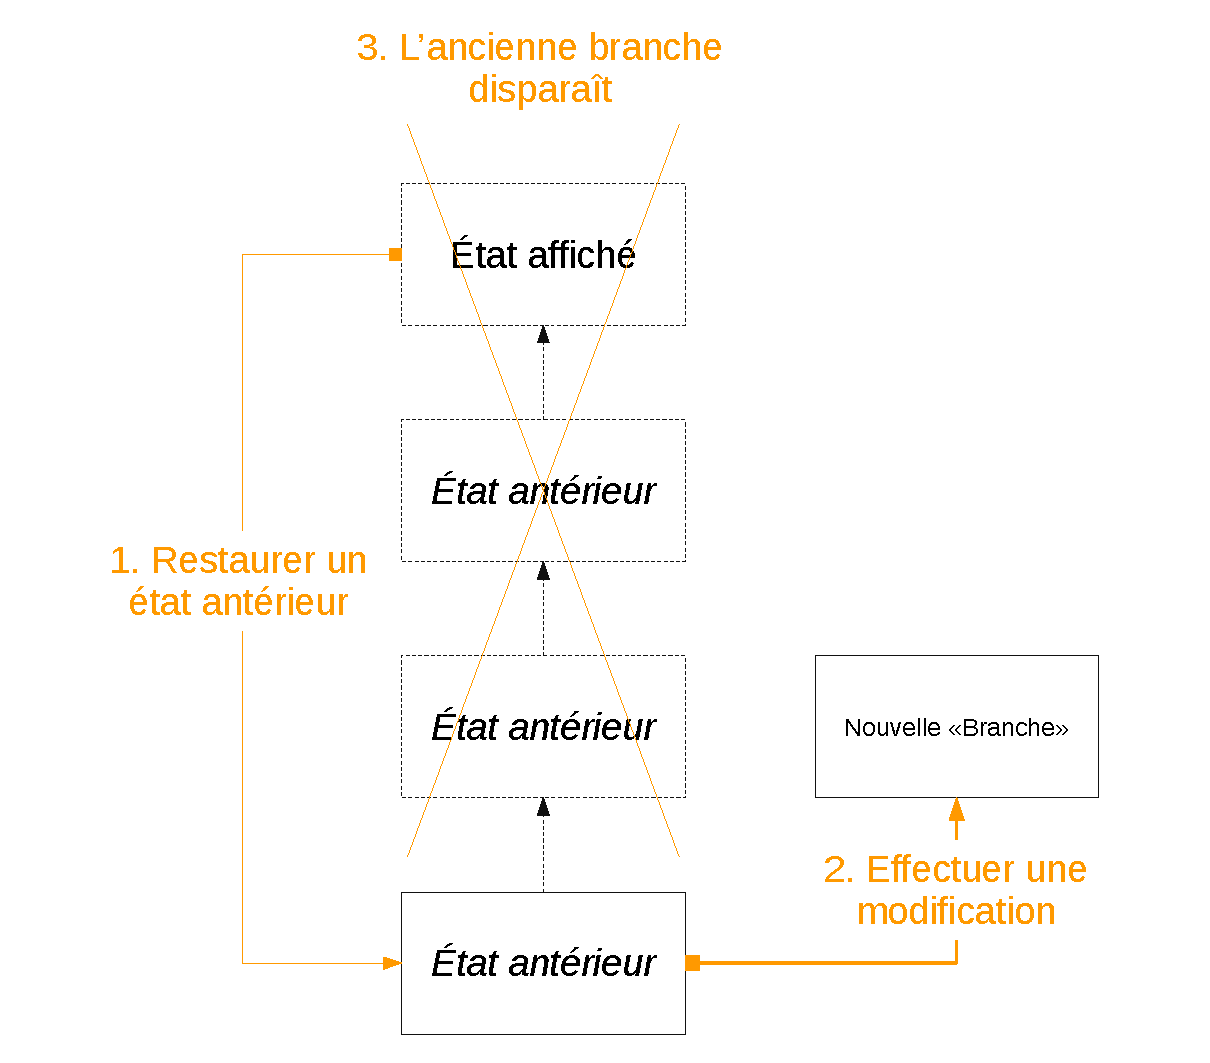
\includegraphics[scale=0.6]{history_branches.pdf}
    \label{fig:hist_branches}
\end{figure}

\subsection{Positionnement}
TODO TODO TODO

\subsection{Outils}
\par
JavaFX offre (entre autres) les événements MousePressed, MouseDragged et MouseReleased. Ils correspondent respectivement à l'action de presser la souris, de la déplacer en gardant le clic gauche enfoncé ou de relâcher le clic gauche de la souris.
\subsubsection{Hiérarchie des outils}
\par
La plupart des outils de l'application  fonctionnent grâce à ces trois événements. On pensera notamment au pinceau qui doit dessiner un trait en suivant la souris lors d'un MouseDragged.
\par
Comme on peut le voir sur la figure \ref{fig:tool_hier}, les outils implémentent une interface Tool, possédant des méthodes correspondant à ces événements. Au long de l'exécution du programme, le Workspace garde une référence vers un outil considéré actif (qui peut aussi être référence nulle), et lorsqu'il détecte un des événements cités plus haut, il se charge d'appeler la ou les méthodes correspondantes de cet outil.
\par
Lorsque l'utilisateur clique sur un bouton pour activer un outil, le programme crée une nouvelle instance de ce type d'outil, et le Workspace utilise cet outil pour traiter les événement MousePressed, MouseDragged ou MouseReleased.
\par
D'autres outils plus simples, comme la symétrie horizontale ou verticale ou les effets de couleurs sont implémentés en ajoutant un action à des composants de bases de JavaFX comme des Button ou des Slider.

\begin{figure}[H]
	\caption{Diagramme simplifié de la hiérarchie des outils}
	\centering
	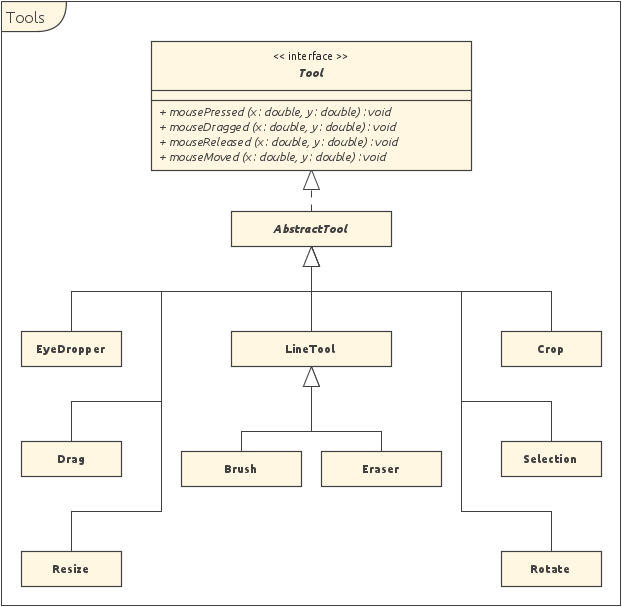
\includegraphics[scale=0.6]{tool_hierarchy.png}
	\label{fig:tool_hier}
\end{figure}

\subsubsection{Réglage des outils} \label{reglage-outils}
Certains de ces outils nécessitent d'être paramétrés en temps réel en fonction des calques sélectionnés par l'utilisateur. Par exemple, la taille de la gomme est stockée dans l'objet représentant l'outil, et est utilisée pour déterminer la taille du rectangle à effacer. L'utilisateur peut la régler au moyen d'un Slider (il s'agit d'un composant JavaFX). Les même besoin concernent la gestion de la couleur du pinceau, de la taille et de la police de l'outil de modification de texte. La figure \ref{fig:text_settings} illustre l'apparence des réglages de l'outil de modification de texte.

\begin{figure}[H]
	\caption{Composant de réglages de l'outil de modification texte}
	\centering
	
\includegraphics[scale=0.6]{toolSettings.png}
	\label{fig:text_settings}
\end{figure}

\par
Ces réglages doivent pouvoir s'adapter à un outil existant, comme par exemple récupérer la taille actuelle du pinceau et la garder en mémoire.

Pour ce faire, les réglages sont gérés au moyen d'une hiérarchie de classes (se référer à la figure \ref{fig:tool_settings}), qui sont en fait des spécialisations de composants JavaFX permettant à l'utilisateur de paramétrer les outils, et d'une série d'interfaces représentant des outils pouvant être paramétrés sur divers aspects (la taille, la couleur, la police et ainsi de suite).
\par
Ainsi un objet ToolFontSettings permet de paramétrer la Font (les paramètres de police d'écriture) d'un objet implémentant l'interface FontConfigruableTool. Dans le cas de l'outil texte, qui implémente cette interface, les réglages doivent s'adapter aux paramètres d'un calque texte et ainsi se mettre à jour en temps réel.
\par
Lorsque l'utilisateur modifie la valeur du Slider contenu dans l'objet ToolFontSettings, celui-ci met à jour sa cible SizeConfigurableTool en temps réel (ici, l'outil de modification de texte).

\begin{figure}[h]
	\caption{Diagramme simplifié des réglages d'outils}
	\centering
	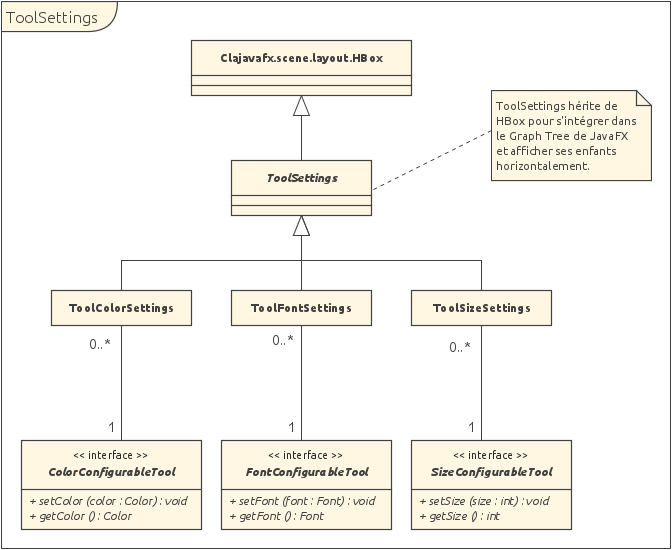
\includegraphics[scale=0.6]{tool_settings.png}
	\label{fig:tool_settings}
\end{figure}

\subsubsection{Pinceau et gomme}
Le pinceau et la gomme ont un comportement et une implémentation quasiment identiques. Dans le programme GEMMS, ce sont les classes Brush et Eraser qui se chargent d'implémenter ces fonctionnalités. Toutes deux héritent d'une classe commune: LineTool.
\par
Pour ces deux outils, la problématique était la suivante:
\par
L'événement MouseDragged est déclenché à intervalles réguliers, tant que l'utilisateur effectue cette action. Pour chaque répétition, il est facile de garder trace de la position de la souris au dernier événement et à l'événement actuel. Connaissant ces deux points, il est possible de dessiner une droite.
\par
Pour ce faire, nous avons utilisé l'algorithme de tracé de segment de Bresenham. Mis au point en 1962, cet algorithme permet de déterminer quels pixels sont à colorer pour relier harmonieusement deux points par une ligne droite.
\par
Il existe de nombreuses implémentations de cet algorithme, et nous avons choisi l'implémentation compacte, que l'on peut trouver sur la page allemande de l'article Wikipédia dédié à ce sujet \cite{Bresenham}.
\par
La classe LineTool se charge donc d'implémenter cet algorithme et pour chaque pixel à colorer, elle appelle une méthode abstraite drawPixel que ses sous classes se chargent de définir. Ainsi, Brush dessiner un disque correspondant à la taille du pinceau, et Eraser efface un carré de pixel, correspondant à la taille de la gomme.
\subsubsection{Pipette}
Le rôle de l'outil pipette est de permettre à l'utilisateur de choisir une couleur en la prélevant sur un élément existant du document. Il s'agirait typiquement de récupérer la couleur d'un calque GEMMSText, GEMMSCanvas ou GEMMSImage.
\par
Dans le cas d'un texte, la pipette retourne simplement la couleur de celui-ci. Dans le cas d'un objet de type GEMMSCanvas ou d'une GEMMSImage, l'outil lit le pixel exact cliqué par l'utilisateur, si celui-ci se trouve à l'intérieur des bornes du calque sélectionné.
\subsubsection{Modification de texte}
L'outil de modification de texte permet à l'utilisateur de modifier les propriétés d'un calque texte existant. Lorsque il clique dessus, si le clic est effectué dans les bornes visuelles du texte, l'outil ouvre une fenêtre de dialogue invitant à changer le contenu du texte.
\par
Les réglages de couleur et de police de cet outils utilisent la structure expliquée à la section \ref{reglage-outils} en utilisant des objets de type ToolColorSettings et ToolFontSettings.
\subsubsection{Symétries}
\subsubsection{Déplacement}
\subsubsection{Rotation}
\subsubsection{Redimensionnement}
\subsubsection{Sélection}
\label{sec:selection}
La sélection permet à l'utilisateur de sélectionner une zone du workspace à l'aide d'un rectangle. Ce dernier peut être déplacer ou recréer si la zone de sélection ne convient pas. 

Pour l'instant, seul le copier coller utilise l'outil de sélection afin de choisir la zone à copier.

\subsubsection{Rognage}
\subsection{Effets}
La section \og Effet \fg{} permet d'appliquer des effets colorimétriques, régler la transparence et ajouter un flou à un ou plusieurs calques. Chaque calque qui doit être modifié passe par une vérification: s'il n'a aucun effet appliqué, on lui applique trois effets: un ColorAdjust, un SepiaTone et un GaussianBlur permettant d'effectuer respectivement des ajustements de la couleur, un effet sépia, et un flou. Ces effets sont initialiement tous réglés pour n'effectuer aucun changement visuel. Ceci permet, lors d'un futur changement des effets, de simplement devoir faire varier les paramètres de ces effets.

\subsubsection{Noir et blanc}
Le bouton \og B\&W \fg{} à pour effet de régler la saturation de l'image à sa valeur minimale, donnant pour effet une image en nuances de gris.

\subsubsection{Tint}
Applique une teinture de la couleur sélectionnée à l'image. Ceci est fait en calculant une valeur de la teinte et en l'appliquant à l'effet ColorAdjust.

\subsubsection{Barres glissantes}
Les barres glissantes (\og Sliders \fg{} JavaFX) permettent d'ajuster tous les autres effets implémentés. La transparence règle directement un attribut \og Opacity \fg{} d'un noeud. La saturation, le contraste et la luminosité peuvent être ajustés en modifiant l'effet ColorAdjust. L'effet sépia et le flou ajustent respectivement l'effet SepiaTone et GaussianBlur.

\subsection{Remise à zéro}
Le bouton \og Reset \fg{} permet de remettre à zéro tous les effets sur tous les calques sélectionnés, les restaurant à leur état visuel initial.
